\documentclass[xcolor=table]{beamer}
\usetheme{CambridgeUS}

\usepackage{amsmath}
\usepackage{xcolor}
\usepackage{hyperref}
\hypersetup{
colorlinks = true,
linkcolor =.,
    citecolor = .,
    urlcolor = blue
}
\usepackage{cancel}
\usepackage{amssymb}
\usepackage{comment}
\usepackage{witharrows}
\usepackage{mathtools}
\usepackage{multicol}

%21-JUN-2016


% Example definitions.
% --------------------

% Specific definitions
\def\Xtr{\mathbf{X}_{\text{tr}}}
\def\Ztr{\mathbf{Z}_{\text{tr}}}

% Packages
\usepackage{bm}
\usepackage{color}
\usepackage{amssymb}

%\usepackage{cite}
%\usepackage[pdftex]{graphicx}
\usepackage{algorithm,algorithmic}
\usepackage{amsmath}
\usepackage{url}
\usepackage{float}
\usepackage{cancel}

\usepackage{multirow}

% Functions
\def\trace{\operatorname{Tr}}
\def\KL{\mathbf{KL}}
\def\PG{\operatorname{PG}}
\newcommand{\E}{\mathbb{E}}

% Number Sets
\def\R{{\mathbb R}}
\def\Z{{\mathbb Z}}
\def\N{{\mathbb N}}

% Text
\def\p{{\mathrm{p}}}
\def\q{{\mathrm{q}}}
\def\rd{{\mathrm{d}}}

\def\F{{\mathrm{F}}}
\def\G{{\mathrm{G}}}
\def\H{{\mathrm{H}}}
\def\T{{\mathrm{T}}}

\def\KL{{\mbox{KL}}}
\def\TV{{\mbox{TV}}}

\def\tr{{\text{tr}}}

% Cal
\def\cC{{\mathcal C}}
\def\cH{{\mathcal H}}
\def\cL{{\mathcal L}}
\def\cN{{\mathcal N}}
\def\cX{{\mathcal X}}

% Bold Symbols and numbers
\def\bzero{{\mathbf 0}}
\def\bone{{\mathbf 1}}

% Greek letters
\def\balpha{{\boldsymbol{\alpha}}}
\def\bbeta{{\boldsymbol{\beta}}}
\def\bgamma{{\boldsymbol{\gamma}}}
\def\bdelta{{\boldsymbol{\delta}}}
\def\bepsilon{{\boldsymbol{\epsilon}}}
\def\bheta{{\boldsymbol{\eta}}}
\def\btheta{{\boldsymbol{\theta}}}
\def\biota{{\boldsymbol{\iota}}}
\def\bkappa{{\boldsymbol{\kappa}}}
\def\blambda{{\boldsymbol{\lambda}}}
\def\bmu{{\boldsymbol{\mu}}}
\def\bnu{{\boldsymbol{\nu}}}
\def\bxi{{\boldsymbol{\xi}}}
\def\bpi{{\boldsymbol{\pi}}}
\def\brho{{\boldsymbol{\rho}}}
\def\bsigma{{\boldsymbol{\sigma}}}
\def\btau{{\boldsymbol{\tau}}}
\def\bups{{\boldsymbol{\upsilon}}}
\def\bphi{{\boldsymbol{\phi}}}
\def\bchi{{\boldsymbol{\chi}}}
\def\bpsi{{\boldsymbol{\psi}}}
\def\bomega{{\boldsymbol{\omega}}}

\def\bAlpha{{\boldsymbol{\Alpha}}}
\def\bBeta{{\boldsymbol{\Beta}}}
\def\bGamma{{\boldsymbol{\Gamma}}}
\def\bDelta{{\boldsymbol{\Delta}}}
\def\bEpsilon{{\boldsymbol{\Epsilon}}}
\def\bHeta{{\boldsymbol{\Eta}}}
\def\bTheta{{\boldsymbol{\Theta}}}
\def\bIota{{\boldsymbol{\Iota}}}
\def\bKappa{{\boldsymbol{\Kappa}}}
\def\bLambda{{\boldsymbol{\Lambda}}}
\def\bMu{{\boldsymbol{\Mu}}}
\def\bNu{{\boldsymbol{\Nu}}}
\def\bXi{{\boldsymbol{\Xi}}}
\def\bPi{{\boldsymbol{\Pi}}}
\def\bRho{{\boldsymbol{\Rho}}}
\def\bSigma{{\boldsymbol{\Sigma}}}
\def\bTau{{\boldsymbol{\Tau}}}
\def\bUps{{\boldsymbol{\Upsilon}}}
\def\bPhi{{\boldsymbol{\Phi}}}
\def\bChi{{\boldsymbol{\Chi}}}
\def\bPsi{{\boldsymbol{\Psi}}}
\def\bOmega{{\boldsymbol{\Omega}}}

% Bold
\def\ba{{\mathbf a}}
\def\bb{{\mathbf b}}
\def\bc{{\mathbf c}}
\def\bd{{\mathbf d}}
\def\be{{\mathbf e}}
\def\bff{{\mathbf f}}
\def\bg{{\mathbf g}}
\def\bh{{\mathbf h}}
\def\bi{{\mathbf i}}
\def\bj{{\mathbf j}}
\def\bk{{\mathbf k}}
\def\bl{{\mathbf l}}
\def\bm{{\mathbf m}}
\def\bn{{\mathbf n}}
\def\bo{{\mathbf o}}
\def\bp{{\mathbf p}}
\def\bq{{\mathbf q}}
\def\br{{\mathbf r}}
\def\bs{{\mathbf s}}
\def\bt{{\mathbf t}}
\def\bu{{\mathbf u}}
\def\bv{{\mathbf v}}
\def\bw{{\mathbf w}}
\def\bx{{\mathbf x}}
\def\by{{\mathbf y}}
\def\bz{{\mathbf z}}

\def\bA{{\mathbf A}}
\def\bB{{\mathbf B}}
\def\bC{{\mathbf C}}
\def\bD{{\mathbf D}}
\def\bE{{\mathbf E}}
\def\bF{{\mathbf F}}
\def\bG{{\mathbf G}}
\def\bH{{\mathbf H}}
\def\bI{{\mathbf I}}
\def\bJ{{\mathbf J}}
\def\bK{{\mathbf K}}
\def\bL{{\mathbf L}}
\def\bM{{\mathbf M}}
\def\bN{{\mathbf N}}
\def\bO{{\mathbf O}}
\def\bP{{\mathbf P}}
\def\bQ{{\mathbf Q}}
\def\bR{{\mathbf R}}
\def\bS{{\mathbf S}}
\def\bT{{\mathbf T}}
\def\bU{{\mathbf U}}
\def\bV{{\mathbf V}}
\def\bW{{\mathbf W}}
\def\bX{{\mathbf X}}
\def\bY{{\mathbf Y}}
\def\bZ{{\mathbf Z}}

% Commands
%--------------------
\newcommand{\mean}[1]{\mathrm{<}#1\mathrm{>}}


%\newcommand{\d}{{\mathrm d}}
\DeclareMathOperator*{\diag}{diag}


% Theorems

\usepackage{amsthm}
\theoremstyle{definition}

\newtheorem{proposition}[]{Proposition}
%\newtheorem{problem}[]{Problem}

\usepackage{arydshln}
\usepackage{natbib}
 


\DeclarePairedDelimiter\abs{\lvert}{\rvert}%
\DeclarePairedDelimiter\norm{\lVert}{\rVert}%

\begin{document}

\title[Ensembles: Combining Label Outputs ]{Ensembles: Combining Label Outputs }
\author[Javier Sáez]{\textbf {Javier Sáez}} % auteur
\institute[Universidad de Granada]{\textbf {Universidad de Granada}}
\date{\today}

\begin{frame}
    \maketitle
\end{frame}

\begin{frame}{Index}
    \tableofcontents
\end{frame}

%%%%%%%%%%%%%%%%%%%%
%%%%%% SECTION %%%%%
%%%%%%%%%%%%%%%%%%%%

\begin{comment}
    
\begin{frame}{Notation}
\begin{itemize}
    \item \(D\) is a classifier (may have a sub-index)
    \item \(E_{i,j}\) refers to the error of the classifier \(i\) in the partition/dataset \(j\).
\end{itemize}

\vspace{1cm}
Book: 
    \cite{10.5555/2935490}
\end{frame}
\end{comment}

%%%%%%%%%%%%%%%%%%%%
%%%%%% SECTION %%%%%
%%%%%%%%%%%%%%%%%%%%
\section{Philosophy and Taxonomy}

\begin{frame}{What is a classifier ensemble?}

\begin{figure}[ht] 
  \label{ fig7} 
  \begin{minipage}[b]{0.5\linewidth}
    \centering
    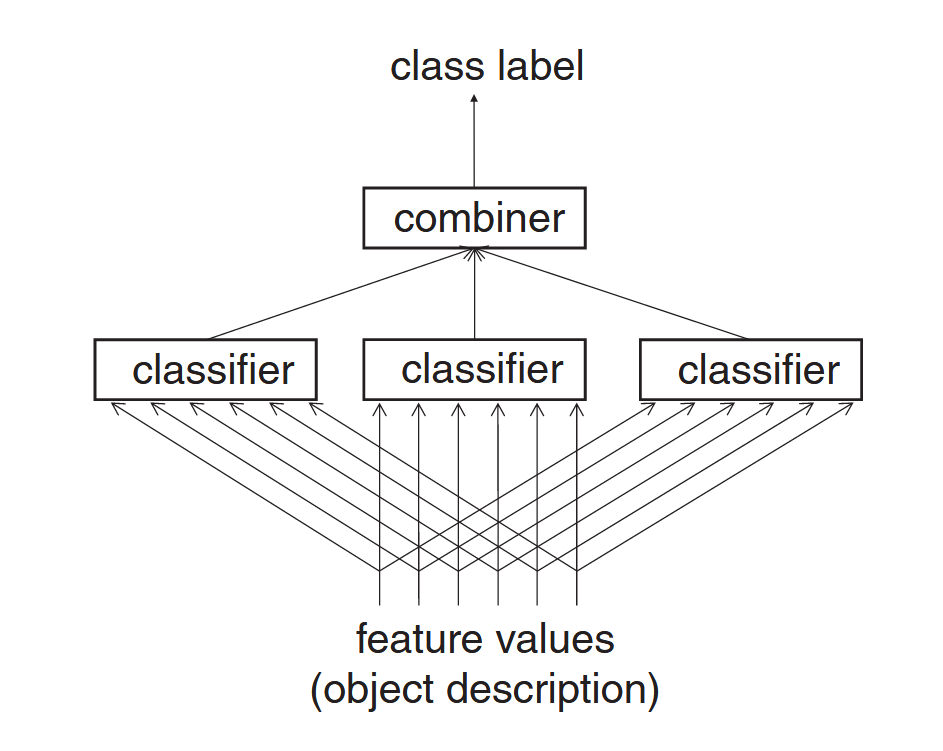
\includegraphics[width=.5\linewidth]{Images/1.png} 
    \caption{Classifier ensemble} 
    \vspace{4ex}
  \end{minipage}%%
  \pause
  \begin{minipage}[b]{0.5\linewidth}
    \centering
    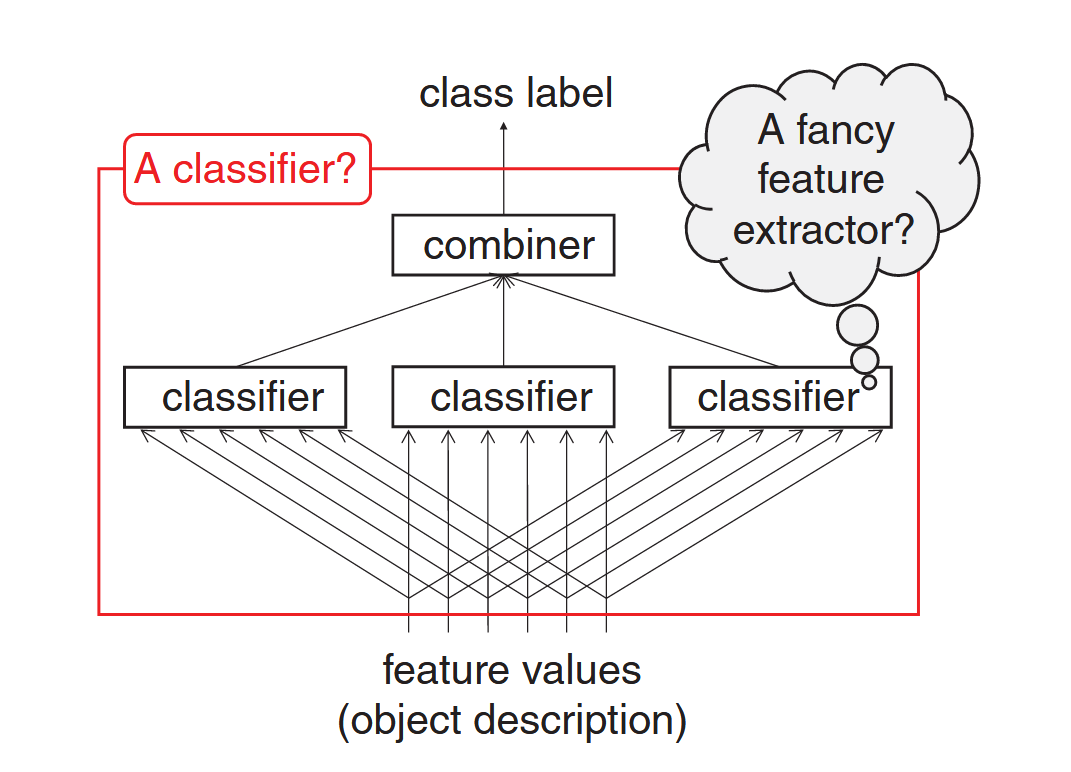
\includegraphics[width=.5\linewidth]{Images/2.png} 
    \caption{¿ Ensemble \(=\) classifier ? (term) } 
    \vspace{4ex}
  \end{minipage} 
  \pause
  \begin{minipage}[b]{0.5\linewidth}
    \centering
    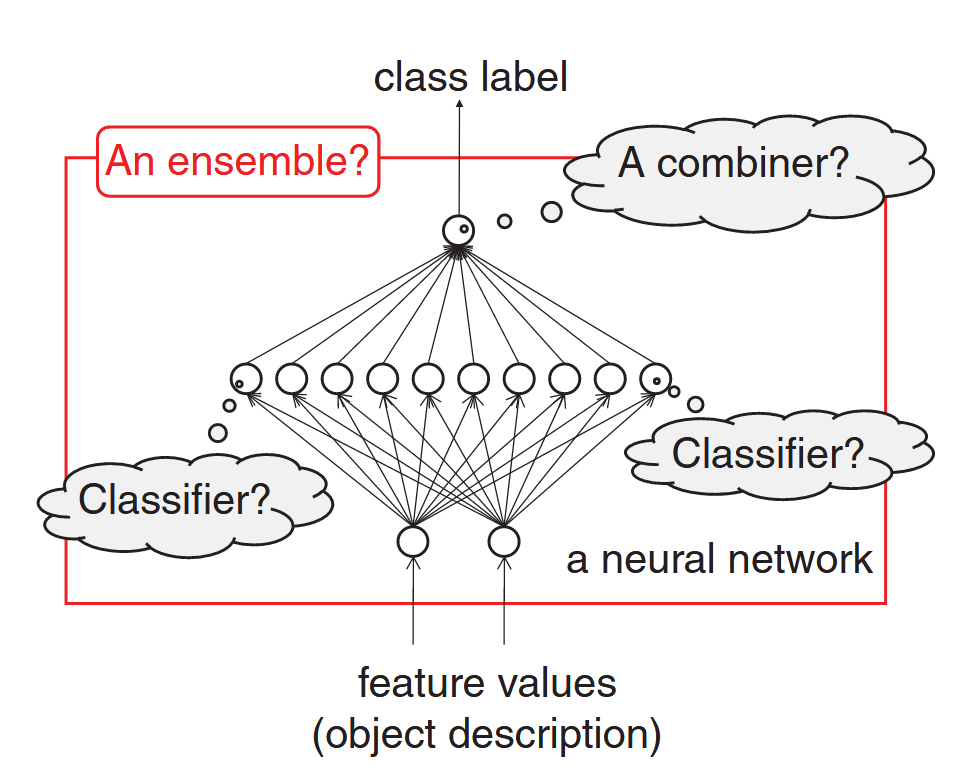
\includegraphics[width=.5\linewidth]{Images/3.png} 
    \caption{¿ NN \(=\) ensemble ?} 
    \vspace{4ex}
  \end{minipage}%% 
  \pause
  \begin{minipage}[b]{0.5\linewidth}
    \centering
    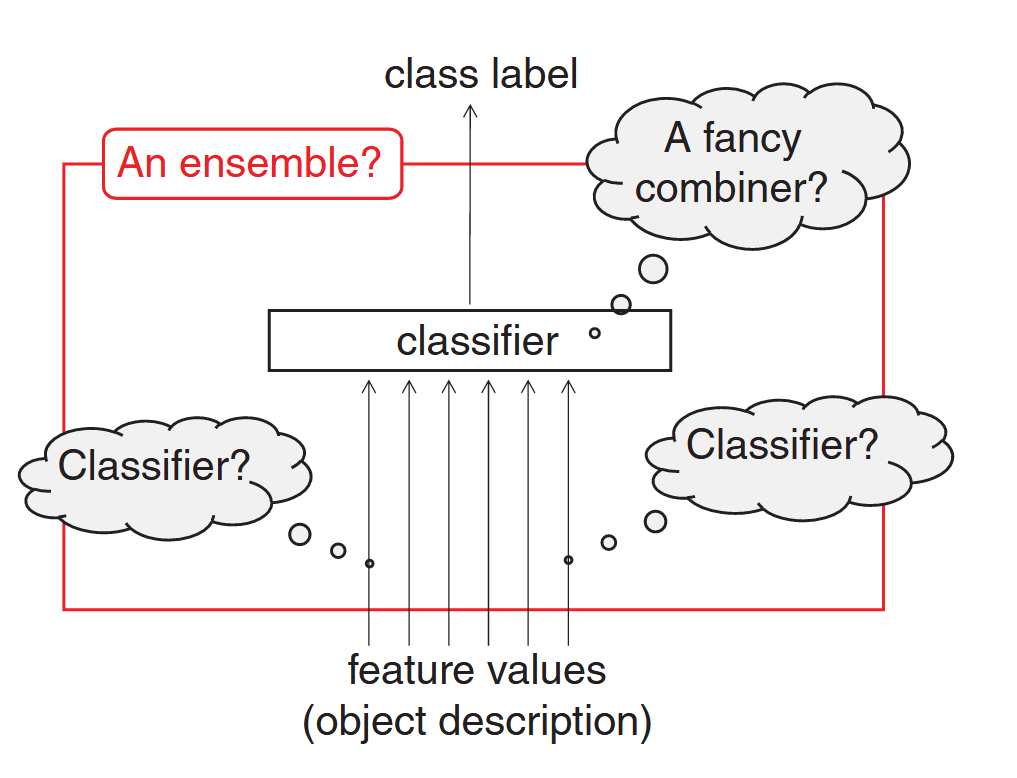
\includegraphics[width=.5\linewidth]{Images/4.png} 
    \caption{¿ Any classifier \(=\) ensemble ?} 
    \vspace{4ex}
  \end{minipage} 
\end{figure}
\end{frame}


\begin{frame}{Why do ensembles work?}
\begin{figure}
\centering
    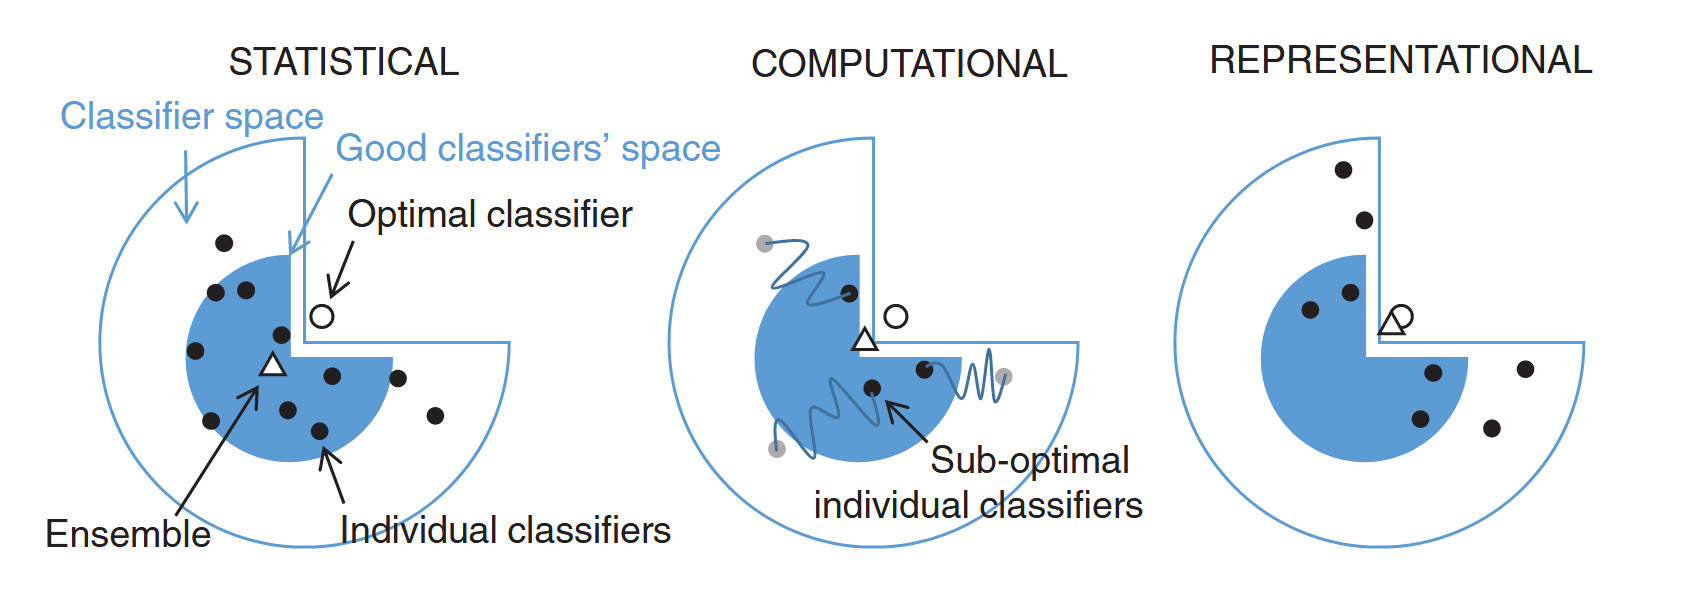
\includegraphics[scale=0.3]{Images/ReasonsEnsemblesWork.png}
    \end{figure}


{\tiny
\begin{columns}
%%%%
\begin{column}{0.3\textwidth}
\textbf{Statistical}\\
\begin{itemize}
    \item Reduce randomness of data and training algorithms
    \item Improve generalization
\end{itemize}

\end{column}
%%%%
\begin{column}{0.3\textwidth} 
\textbf{Computational}\\
\begin{itemize}
    \item Avoid local optima
    \item Split data between classifiers
    \item ¿ Small amount of data ? \(\implies\) Resample
    \item Divide and conquer
\end{itemize}
\end{column}
%%%
\begin{column}{0.3\textwidth}
\textbf{Representational}\\
\begin{itemize}
    \item Approximate boundaries using simpler ones
\end{itemize}
\end{column}
\end{columns}
}
\end{frame}


\begin{frame}{Taxonomy}
    \begin{itemize}
        \item \textbf{Combiner}: Non trainable/Trainable/Meta-classifier
        \item \textbf{Training the ensemble}: Independent/Incremental training
        \item \textbf{Diversity}:
        \begin{itemize}
            \item Training of base classifiers
            \item Resampling data
            \item Partitioning data
            \item Different base models
            \item Different labels
        \end{itemize}
        \item \textbf{Ensemble size}: Fixed in advance/during training/overproduce
        \item \textbf{Universality}: Specified/Any base classifier model
    \end{itemize}
\end{frame}


\begin{frame}{Combination Overview}
    \begin{figure}
        \centering
        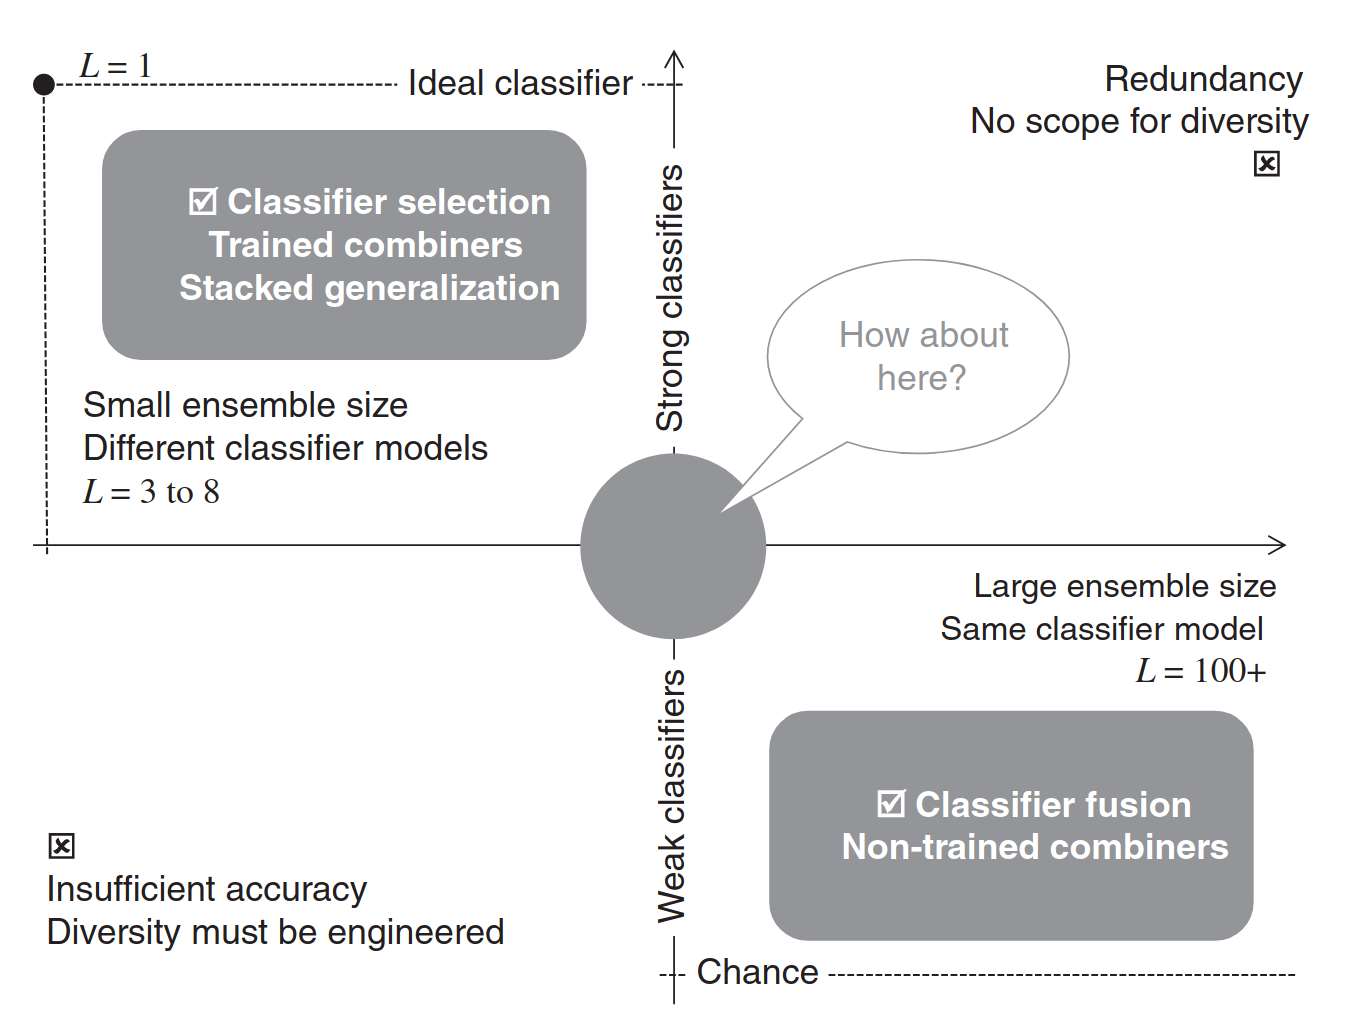
\includegraphics[scale=0.15]{Images/CombinationApproaches.png}
        \caption{Summary of popular classifier combination approaches.}
    \end{figure}
\end{frame}

%%%%%%%%%%%%%%%%%%%%
%%%%%% SECTION %%%%%
%%%%%%%%%%%%%%%%%%%%

\section{Combining Label Outputs}

\begin{frame}{Types of outputs}
    Consider \(\mathbf{\mathcal D} = \{D_i\}_{i=1}^L\) and a set of classes \(\mathbf{\Omega} = \{\omega_i\}_{i=1}^c\). Labels can be:
    \pause
    \begin{itemize}
        \item Class label: \(D_i: \R^n \to \mathbf{\Omega}\) and the \(L\) classifiers define a vector \(\bs = [s_1,\dots,s_L]^T \in \mathbf{\Omega}^L\).
        \pause
        \item Ranked class labels: \(D_i: \R^n \to \mathbf{\Omega}^k \), suitable for large number of classes.
        \pause
        \item Numerical support for classes: \(D_i:\R^n \to [0,1]^c\). We create a matrix \(\mathbf D\) where \(d_{i,j}\) is the support value that classifier \(i\) assigns \(\bx\) to belong to class \(j\). 
        \pause
        \item Oracle: We only consider if the classifier is correct or wrong: \(D_i: \R^n \to \{1,0\}\),  where \(1\) indicates that \(D_i\) classified \(\bx\) correctly.
    \end{itemize}
\end{frame}

\subsection{Probabilistic framework}

\begin{frame}{Probabilistic framework}
    Given \(\bs = [s_1,\dots,s_L]^T\), we are interested in
    \[
    p(\omega_k \mid \bs), \quad k=1,\dots,c.
    \]
    We \textbf{assume} that the classifier give \textbf{independent} decissions, \textbf{conditioned upon the class label}:
    \[
    p(\bs \mid \omega_k) = p(s_1\mid \omega_k) \dots p(s_L\mid \omega_k).
    \]
    \pause
    Using Bayes rule
    \begin{align*}
    p(\omega_k \mid \bs) & = \frac{p(\bs \mid \omega_k) p(\omega_k)}{p(\bs)} = \frac{p(\omega_k)}{p(\bs)} \prod_{i=1}^L p(s_i \mid \omega_k) \\
    & = \frac{p(\omega_k)}{p(\bs)} \times \prod_{i\in I^k_+} p(s_i \mid \omega_k) \times \prod_{i\in I^k_-} p(s_i \mid \omega_k)
    \end{align*}
    
\end{frame}

%%%%%%%%%%%%%%%%%%%%
%%%%%% SECTION %%%%%
%%%%%%%%%%%%%%%%%%%%

\subsection{Majority Vote}
\begin{frame}{Majority Vote}
\begin{figure}
    \centering
    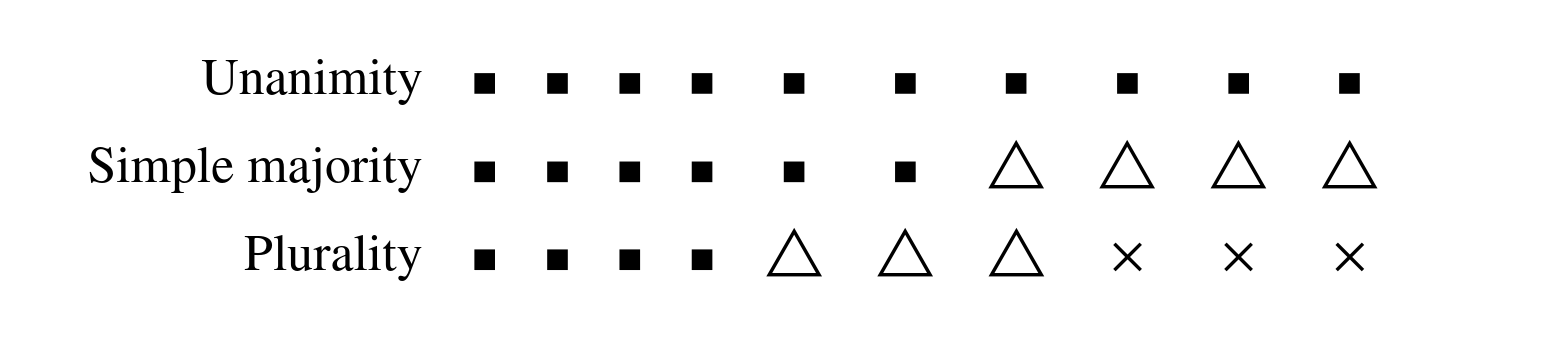
\includegraphics[scale=0.18]{Images/MajorityVote}
    \label{fig:my_label}
\end{figure}
Considering \(d_{i,j} = 1\) if \(D_i\) labels \(\bx\) in \(\omega_j\) and \(0\) otherwise, the \textbf{plurality vote} (\emph{a.k.a. majority vote}) returns \(\omega_k\) if
\[
\sum_{i=1}^L d_{i,k} = \max_{j=1}^c \sum_{i=1}^L d_{i,j}.
\]
\textbf{Thresholded majority vote} adds a needed confidence for the vote to be valid:
\[
\begin{cases}
    \omega_k, & \text{if } \sum_{i=1}^L d_{i,j} \geq \alpha L \\
    \omega_{c+1}, & \text{otherwise}
\end{cases}
\]
with \(0 < \alpha \leq 1\).
    
\end{frame}

\begin{frame}{Accuracy of Majority Vote}

Assuming:
\begin{itemize}
    \item The number of classifiers \(L\) is odd.
    \item Each classifiers assigns the correct class label with a probability \(p\) for any input.
    \item The classifier outputs are independent.
\end{itemize}

Majority vote will give an accurate class label if \textbf{at least} \(\lfloor L/2 \rfloor + 1\) classifiers give correct answers. Then, the accuracy of the ensemble is:
\begin{equation}
p_{maj} = \sum_{\lfloor L/2\rfloor + 1}^L \binom{L}{m} p^m (1-p)^{L-m}
\end{equation}
\end{frame}

\begin{frame}{Condorcet Jury Theorem}
\begin{theorem}[Condorcet Jury Theorem]
    In the previously presented conditions:
    \begin{enumerate}
        \item If \(p > 0.5\), then \(p_{maj}\) is monotonically increasing and 
        \[
        p_{maj}\to 1 \quad \text{as} \quad L \to \infty.
        \]
        \item If \(p < 0.5\) then \(p_{maj}\) is monotonically decreasing and
        \[
        p_{maj}\to 0 \quad \text{as} \quad L \to \infty.
        \]
        \item If \(p = 0.5\), then \(p_{maj} = 0.5\) for any \(L\).
    \end{enumerate}
\end{theorem}
    
\end{frame}

\begin{frame}{Pattern of success}
    \textbf{Intuitively:} Best improvement over individual accuracy is achieved when exactly \(\lfloor L/2\rfloor + 1\) votes are correct. Extras are wasted.

\pause
    \begin{definition}[Pattern of success]
        The \textbf{pattern of success} is a distribution of the \(L\) classifier outputs such that:
        \begin{itemize}
            \item The probability of any combination of \(\lfloor L/2\rfloor + 1\) correct and \(\lfloor L/2\rfloor\) incorrect is \(\alpha\).
            \item The probability of all votes being incorrect is \(\gamma\).
            \item Any other combination has probability \(0\).
        \end{itemize}
    \end{definition}
    \pause
    In this scenario, the accuracy of the ensemble is:
    \[
    p_{maj} = \min \left\{1, \frac{2pL}{L+1}\right\}
    \]
\end{frame}


\begin{frame}{Pattern of failure}
    \begin{definition}[Pattern of failure]
        The \textbf{pattern of failure} is a distribution of the \(L\) classifier outputs such that:
        \begin{itemize}
            \item The probability of any combination of \(\lfloor L/2\rfloor\) correct and \(\lfloor L/2\rfloor + 1\) incorrect is \(\beta\).
            \item The probability of all votes being correct is \(\delta\).
            \item Any other combination has probability \(0\).
        \end{itemize}
    \end{definition}
    \pause
    In this scenario, the accuracy of the ensemble is:
    \[
    p_{maj} = \frac{(2p-1)L + 1}{L+1}
    \]
\end{frame}

\begin{frame}{Matan's bounds on the Majority Vote Accuracy}
        Consider that classifier \(D_i\) has accuracy \(p_i\) and \(\{D_1,\dots,D_L\}\) are arranged so that \(p_1\leq p_2\leq \dots \leq p_L\). Let \(k = (L+1)/2\). Then the accuracy of the majority vote ensemble has the following lower and upper bounds:
        \[
           \max \{0, \xi(k),\xi(k-1),\dots,\xi(1)\}\leq p_{maj} \leq \min \{ 1, \Sigma(k),\Sigma(k-1),\dots, \Sigma(1)\}
            \]
            where
            \[
            \Sigma(m) = \frac{1}{m}\sum_{i=1}^{L-k+m}p_i, \quad m = 1,\dots,k,
            \]
            and
            \[
            \xi(m) = \frac{1}{m} \sum_{i=k-m+1}^L p_i - \frac{L-k}{m},\quad m=1,\dots,k
            \]

\end{frame}

\begin{frame}{Optimality of the Majority Vote Combiner}
    \begin{theorem}
        Let \(\mathbf{\mathcal D}\) be an ensemble of \(L\) classifiers. Suppose that:
        \begin{enumerate}
            \item The classifiers give their decisions independently, conditioned upon the class label.
            \item The individual classification accuracy is \(p\) for all the classifiers, classes and datapoints.
            \item The probability for incorrect classification is equally distributed among the remaining classes:
            \[
            P(s_i = \omega_j \mid \omega_k) = \frac{1-p}{c-1}, \quad i =1,\dots,L; \ k,j = 1,\dots,c \ j \neq k
            \]
        \end{enumerate}
        Then, the majority vote is the optimal combination rule.
    \end{theorem}
\end{frame}

%%%%%%%%%%%%%%%%%%%%
%%%%%% SECTION %%%%%
%%%%%%%%%%%%%%%%%%%%

\subsection{Weighted Majority Vote }

\begin{frame}{Weighted Majority Vote (WMV)}
    If the classifiers in the ensemble do not have identical accuracy, it is reasonable to give the more competent classifiers more power in the final decision. \\
    Using the previous \(d_{i,j}\), the \textbf{class-support} function for class \(\omega_j\) obtained through weighted voting is:
    \[
    \mu_j(\bx) = \sum_{i=1}^L b_i d_{i,j},
    \]
    where \(b_i\) is a coefficient for classifier \(D_i\).\\

    The value of this function will be the sum of the weights for the classifiers of the ensemble whose output for \(\bx\) is \(\omega_j\).
\end{frame}


\begin{frame}{Optimality of Weighted Majority Vote}

    \begin{theorem}
        Let \(\mathbf{\mathcal D}\) be an ensemble of \(L\) classifiers. Suppose that:
        \begin{itemize}
            \item The classifiers give their decisions independently, conditioned upon the class label.
            \item The individual classification accuracy is \(p_i\) for any class \(\omega_k\) and any datapoint. {\color{brown} (We relax the assumption about equal individual accuracies)}
            \item The probability for incorrect classification is equally distributed among the remaining classes.
        \end{itemize}
        Then the WMV is the optimal combination rule with weights:
        \begin{equation}
            b_i = \log \left( \frac{p_i}{1-p_i}\right), \quad 0 \leq p_i \leq 1
        \end{equation}
    \end{theorem}
\end{frame}
%%%%%%%%%%%%%%%%%%%%
%%%%%% SECTION %%%%%
%%%%%%%%%%%%%%%%%%%%

\subsection{Naïve Bayes Combiner}
\begin{frame}{Naïve Bayes Combiner}
    \begin{definition}[Naïve Bayes Classifier]
        Given an unknown sample \(\bx^\star\), the \emph{Naive Bayes (NB) \textbf{classifier}} assigns the sample a label according to the \emph{maximum a posteriori} decision rule:
        \[
        y^\star = \arg \max_{k} p(\omega_k) \prod_{i=1}^L p(x_i \mid \omega_k)
        \]
    \end{definition}
    The Naïve Bayes \textbf{combiner} applies the NB classifier in the case where the input \(\bx^\star\) is a vector of the outputs of each of the classifiers.\\

\pause

    \emph{Implementation detail: In practise, the probabilities are estimated by computing a confusion matrix for each of the classifiers using the whole dataset.}
    \[
    p(s_i \mid \omega_k) = \frac{cm^i_{k,s_i}}{N_k}, \quad p(\omega_k) = \frac{N_k}{N}
    \] 

\end{frame}


\begin{frame}{Optimality of the Naïve-Bayes Combiner}
    \begin{theorem}
        Let \(\mathbf{\mathcal D}\) be an ensemble of \(L\) classifiers. Suppose that the classifiers give their decisions independently, conditioned upon the class label. Then, the Naïve Bayes combiner 
        \[
        \omega^\star = \max \left\{p(\omega_k) \prod_{i=1}^L p(s_i \mid \omega_k)\right\}
        \]
        is the optimal combination rule.
    \end{theorem}
\end{frame}


%%%%%%%%%%%%%%%%%%%%
%%%%%% SECTION %%%%%
%%%%%%%%%%%%%%%%%%%%

\subsection{Behavior Knowledge Space}

\begin{frame}{Behavior Knowledge Space (BKS)-\citep{BKS1995}}

A  \textbf{Behaviour Knowledge Space} is a \(L-\) dimensional space where each dimension correspond to the decision of one classifier.\\
\pause

    Consider \(\bx \in \R^n\) and \(\bs_\bx = [s_1,\dots,s_L]^T\) the labels asigned by each of the \(L\) classifiers to \(\bx\). Consider also:
    \begin{itemize}
        \item \(\bE \in \mathcal M_{N\times L}\), where the i-th row \(\bE_i\) contains the vector \(\bs_{\bx_i}\) of the training set.
        \item \(\bT \in \mathcal M_{N\times 1}\), the vector of the true labels of the training set.
        \item \(\omega_p\) is the most represented class in \(\bT\).
        \item \(R(\bS)\) is the most represented class in the set \(\bS\). Also, \(n_\bS(k)\) is the number of times that class \(k\) is in \(\bS\).
    \end{itemize}
\end{frame}

\begin{frame}{BKS Algorithm}

\begin{algorithm}[H]
\begin{algorithmic}[1]

\STATE \(\bS = \{\emptyset\}\)
\STATE Compute \(\br = [D^1(\bx^\star),\cdots,D^L(\bx^\star)]\)
\FOR{Each each row \(\bE_i\) of \(\bE\)}
\IF{\(\br == \bE_i\)}
\STATE \(\bS = \bS \cup \{\bT_i\}\)
\ENDIF
\ENDFOR
\IF{\(\bS == \{\emptyset\}\)}
\RETURN \(\omega_p\) or \(\omega_{C+1}\)
\ELSE
\RETURN \(R(\bS)\)
\ENDIF
\end{algorithmic}
\caption{BKS Combiner}
\label{alg:seq}
\end{algorithm}
\end{frame}


\begin{frame}{BKS: Confidence Variant}

Let \(\abs{\bS}\) be the cardinal of \(\bS\) and \(E(\bx^\star)\) be the output of the BKS method. Considering a confidence level \(0 < \lambda < 1\), BKS can return:
\[
E(\bx^\star) = \begin{cases}
   R(\bS) & \text{If } \abs{\bS} > 0  \text{ and } \frac{n_\bS(R(\bS))}{\abs{S}} \geq \lambda\\
   \omega_p \text{ or } \omega_{C+1} & \text{otherwise}.
\end{cases}
\]

\pause
\begin{alertblock}{Warning}
This method needs a big dataset in order to create a representative BKS.
\end{alertblock}

\end{frame}


%%%%%%%%%%%%%%%%%%%%
%%%%%% SECTION %%%%%
%%%%%%%%%%%%%%%%%%%%

\subsection{Comparison}


\begin{frame}{Comparison}
\begin{figure}
    \centering
    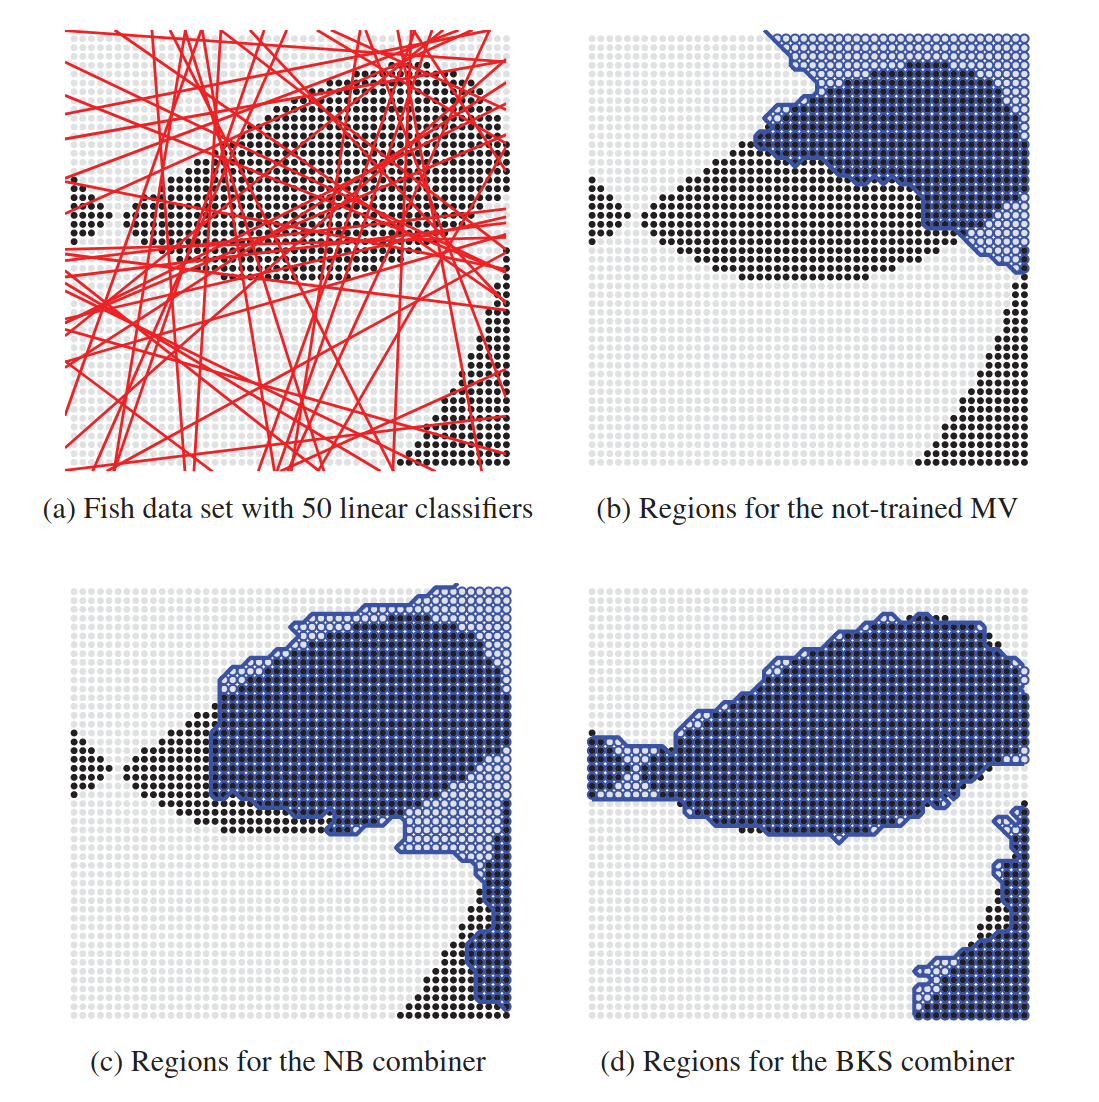
\includegraphics[scale=0.18]{Images/Comparison.png}
    %\caption{Caption}
\end{figure}
    
\end{frame}

\begin{frame}{Comparison}
    % Please add the following required packages to your document preamble:
% \usepackage[table,xcdraw]{xcolor}
% If you use beamer only pass "xcolor=table" option, i.e. \documentclass[xcolor=table]{beamer}
\begin{table}[]
\begin{tabular}{l|llllr}
Combiner               & 1                                               & 2                                               & 3                                               & 4                        & Number of parameters \\ \hline
Majority Vote          & \cellcolor[HTML]{000000}{\color[HTML]{000000} } &                                                 &                                                 &                          & none                 \\
Weighted Majority Vote & \cellcolor[HTML]{000000}{\color[HTML]{000000} } & \cellcolor[HTML]{000000}                        &                                                 &                          & $L+c$                \\
Naive Bayes            & \cellcolor[HTML]{000000}{\color[HTML]{000000} } & \cellcolor[HTML]{000000}{\color[HTML]{000000} } & \cellcolor[HTML]{000000}{\color[HTML]{000000} } &                          & $Lc^2 + c$           \\
BKS                    & \cellcolor[HTML]{000000}                        & \cellcolor[HTML]{000000}                        & \cellcolor[HTML]{000000}                        & \cellcolor[HTML]{000000} & $c^L$               
\end{tabular}
\end{table}
Columns mean \textbf{scopes of optimality}:
\begin{itemize}
    \item Equal \(p\)
    \item Classifier specific \(p_i\)
    \item Full confusion matrix
    \item Independence not required
\end{itemize}
\end{frame}

%%%%%%%%%%%%%%%%%%%%
%%%%%% SECTION %%%%%
%%%%%%%%%%%%%%%%%%%%
\section*{}

\begin{frame}{}
    \begin{center}
        Thank you for your attention
    \end{center}
\end{frame}




  \begin{frame}[noframenumbering]{Bibliography}

  %\vspace{0.5cm}
  \bibliographystyle{unsrtnat}
  \bibliography{bibliography.bib}

  \end{frame}
\end{document}